% Slide 1: Cover
\begin{frame}[plain]
  \begin{center}
    \vspace*{0.6cm}
    
\includegraphics[height=1.2cm]{images/mannheim_logo.png}\\[0.6cm]
    {\fontsize{10}{12}\selectfont\color{subgray}دانشگاه مانهایم $\bullet$ گروه علوم داده و وب}\\[0.4cm]
    {\fontsize{20}{24}\selectfont\color{mannheimblue}\textbf{داده‌کاوی \lr{(IE500)}}}\\[0.3cm]
    {\fontsize{16}{20}\selectfont\color{mannheimteal}\textbf{فصل ششم: خوشه‌بندی \lr{(Clustering)}}}\\[0.8cm]
    {\fontsize{8.5}{11}\selectfont\color{subgray}نسخه \lr{23.03.2025}}
  \end{center}
\end{frame}

% Slide 2: Outline
\begin{frame}{سرفصل مطالب}{\lr{Outline}}
  \begin{itemize}
    \setlength{\itemsep}{8pt}
    \item \textbf{تحلیل خوشه چیست؟} \lr{(What is Cluster Analysis?)}
    \item \textbf{خوشه‌بندی \lr{K-Means}} \lr{(K-Means Clustering)}
    \item \textbf{خوشه‌بندی مبتنی بر چگالی (\lr{DBSCAN})} \lr{(Density-based Clustering - DBSCAN)}
    \item \textbf{معیارهای مجاورت و شباهت} \lr{(Proximity Measures)}
    \item \textbf{تشخیص ناهنجاری و داده‌های پرت} \lr{(Anomaly Detection)}
    \begin{itemize}
      \setlength{\itemsep}{4pt}
      \item رویکردهای آماری \lr{(Statistical Approaches)}
      \item رویکردهای مبتنی بر فاصله و چگالی \lr{(Distance \& Density-based Approaches)}
    \end{itemize}
  \end{itemize}
\end{frame}

% Slide 3: What is Cluster Analysis?
\begin{frame}{تحلیل خوشه چیست؟}{\lr{What is Cluster Analysis?}}
  \begin{itemize}
    \setlength{\itemsep}{4pt}
    \item \textbf{تعریف:} یافتن گروه‌هایی از اشیاء به‌گونه‌ای که اشیاء درون یک گروه:
    \begin{itemize}
      \setlength{\itemsep}{2pt}
      \item \textbf{بسیار شبیه} به یکدیگر باشند \lr{(Intra-cluster similarity)}.
      \item و با اشیاء متعلق به سایر گروه‌ها \textbf{متفاوت} باشند \lr{(Inter-cluster dissimilarity)}.
    \end{itemize}
    \item \textbf{هدف اصلی:} دستیابی به درک و بینش عمیق‌تر از ساختار ذاتی داده‌ها \lr{(Data Understanding)}.
  \end{itemize}
  \vspace{0.1cm}
  \begin{center}
    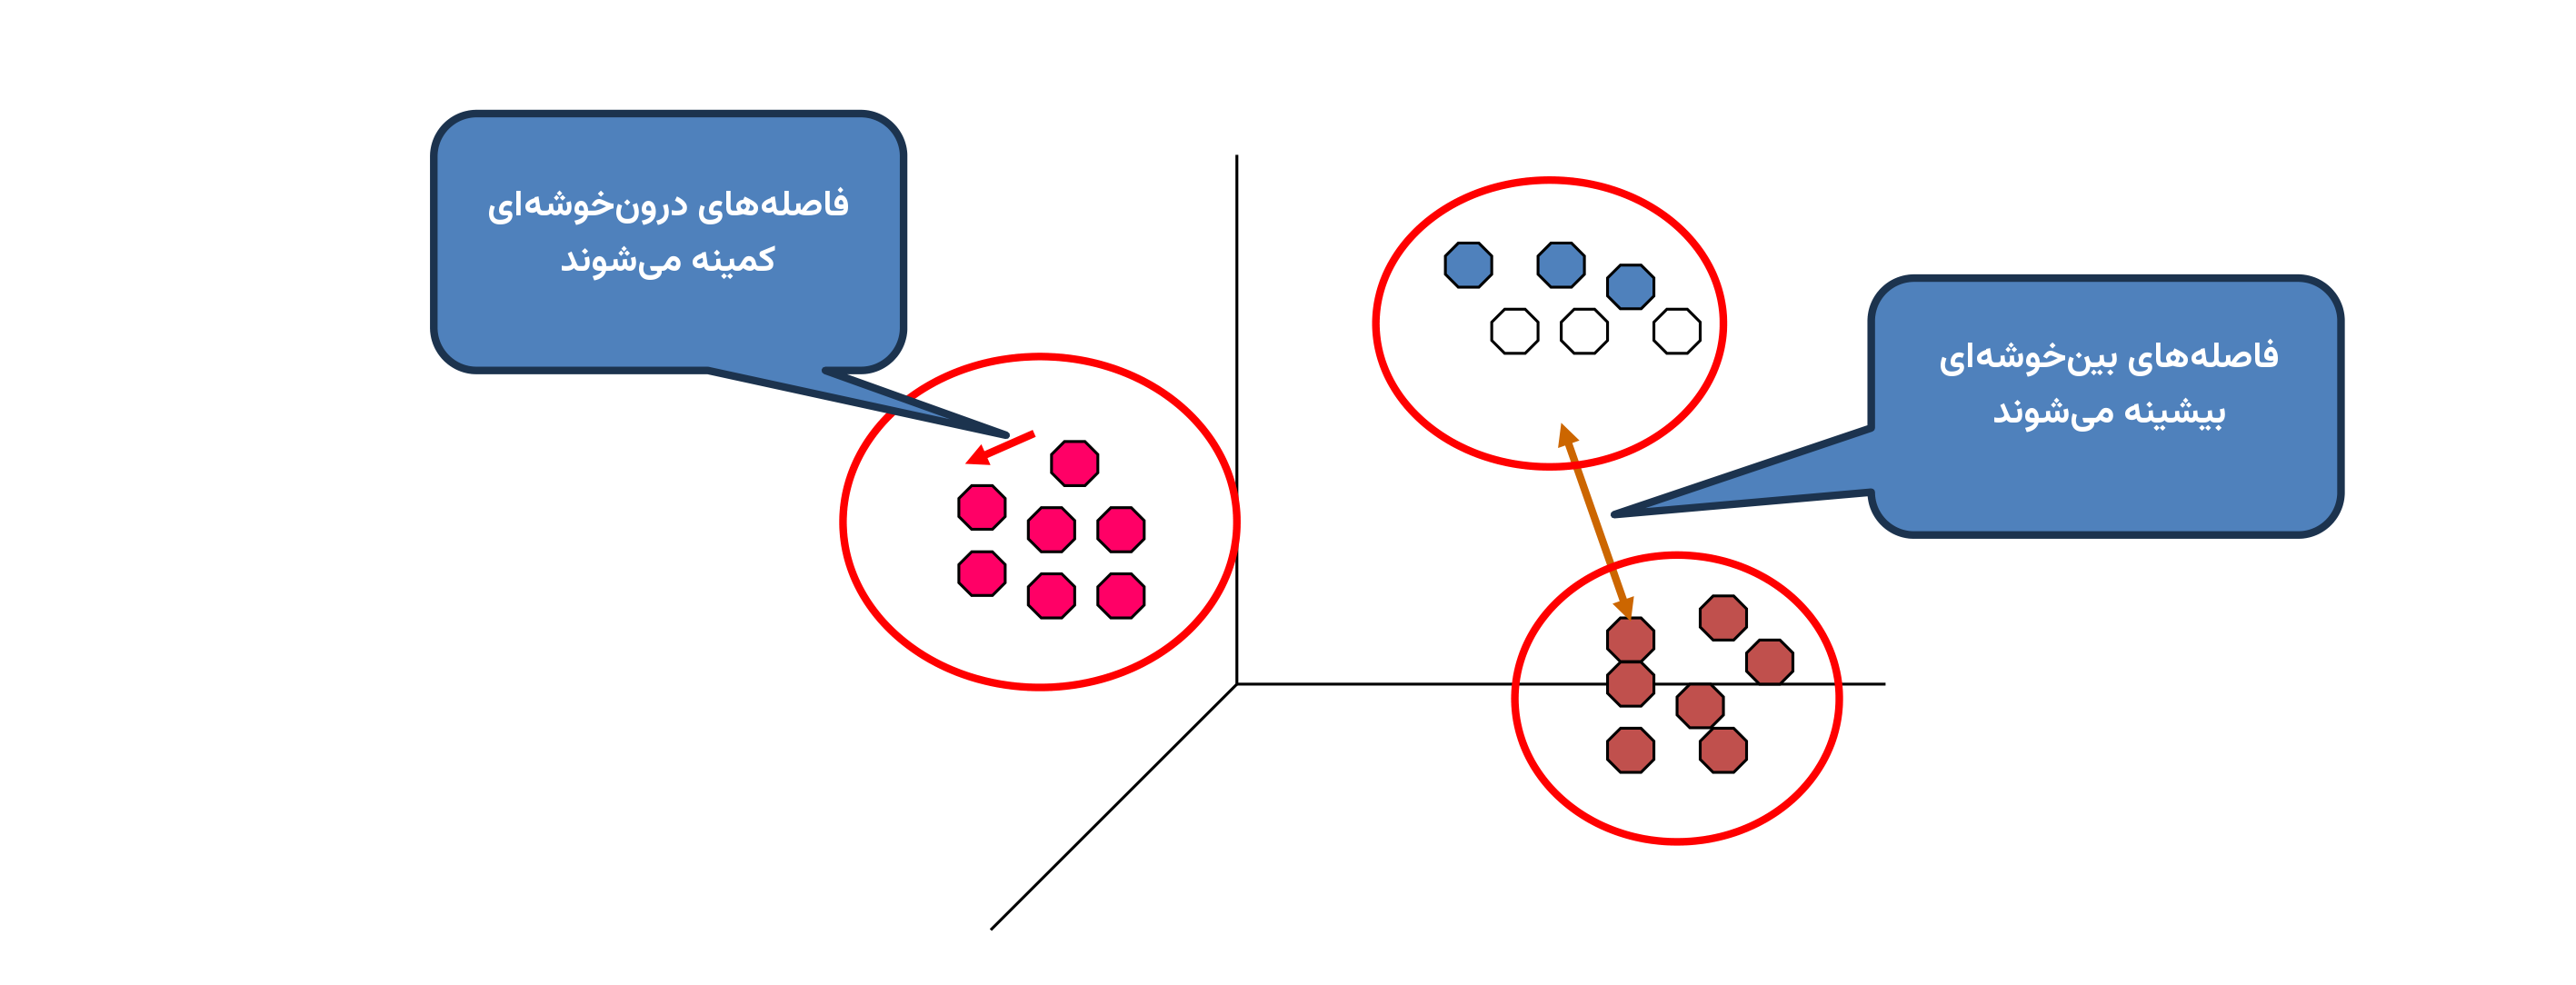
\includegraphics[width=0.75\textwidth,height=3.8cm,keepaspectratio]{images/slide03_diagram_persian.png}
  \end{center}
\end{frame}

% Slide 4: Cluster Analysis as Unsupervised Learning
\begin{frame}{تحلیل خوشه به عنوان یادگیری بدون‌ناظر}{\lr{Cluster Analysis as Unsupervised Learning}}
  \begin{columns}[T]
    \begin{column}{0.48\textwidth}
      \begin{block}{\textbf{یادگیری با‌ناظر \lr{(Supervised)}}}
        \begin{itemize}
          \setlength{\itemsep}{3pt}
          \item کشف الگوهایی برای اتصال ویژگی‌ها به ویژگی هدف \lr{(Target / Class)}.
          \item مجموعه کلاس‌ها از پیش \textbf{معلوم و مشخص} است.
          \item برچسب‌ها توسط ناظر انسانی یا ثبت قبلی ارائه می‌شوند.
          \item هدف اصلی: \textbf{پیش‌بینی} برچسب هدف برای نمونه‌های جدید.
        \end{itemize}
      \end{block}
    \end{column}
    \begin{column}{0.48\textwidth}
      \begin{block}{\textbf{یادگیری بدون‌ناظر \lr{(Unsupervised)}}}
        \begin{itemize}
          \setlength{\itemsep}{3pt}
          \item داده‌ها \textbf{هیچ متغیر هدفی ندارند}.
          \item کاوش در داده‌ها برای کشف ساختارهای ذاتی پنهان \lr{(Intrinsic Structures)}.
          \item دسته‌ها یا خوشه‌ها از قبل شناخته‌شده نیستند.
          \item تحلیل خوشه و استخراج قواعد انجمنی از نمونه‌های برجسته این یادگیری هستند.
        \end{itemize}
      \end{block}
    \end{column}
  \end{columns}
\end{frame}

% Slide 5: Types of Clusterings
\begin{frame}{انواع خوشه‌بندی}{\lr{Types of Clusterings}}
  \begin{columns}[T]
    \begin{column}{0.54\textwidth}
      \begin{itemize}
        \setlength{\itemsep}{7pt}
        \item \textbf{خوشه‌بندی افرازی:} \lr{(Partitional Clustering)}
        \begin{itemize}
          \setlength{\itemsep}{3pt}
          \item تقسیم اشیاء داده به زیرمجموعه‌های غیرهم‌پوشان (خوشه‌ها).
          \item هر شیء دقیقاً متعلق به \textbf{یک زیرمجموعه} است.
        \end{itemize}
        \item \textbf{خوشه‌بندی سلسله‌مراتبی:} \lr{(Hierarchical Clustering)}
        \begin{itemize}
          \setlength{\itemsep}{3pt}
          \item مجموعه‌ای از خوشه‌های تو‌در‌تو که ساختار یک درخت سلسله‌مراتبی \lr{(Dendrogram)} را تشکیل می‌دهند.
        \end{itemize}
      \end{itemize}
    \end{column}
    \begin{column}{0.44\textwidth}
      \begin{center}
        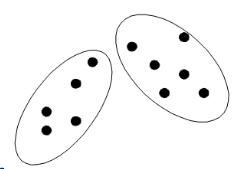
\includegraphics[height=2.0cm,keepaspectratio]{images/slide05_partitional_user.png}\\[0.25cm]
        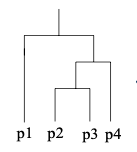
\includegraphics[height=1.9cm,keepaspectratio]{images/slide05_dendrogram_user.png}
      \end{center}
    \end{column}
  \end{columns}
\end{frame}

% Slide 6: Aspects of Cluster Analysis
\begin{frame}{جنبه‌های کلیدی تحلیل خوشه}{\lr{Aspects of Cluster Analysis}}
  \begin{itemize}
    \setlength{\itemsep}{6pt}
    \item \textbf{الگوریتم خوشه‌بندی:} \lr{(Clustering Algorithm)}
    \begin{itemize}
      \setlength{\itemsep}{2pt}
      \item الگوریتم‌های افرازی \lr{(Partitional)} نظیر \lr{K-Means}
      \item الگوریتم‌های مبتنی بر چگالی \lr{(Density-based)} نظیر \lr{DBSCAN}
      \item الگوریتم‌های سلسله‌مراتبی \lr{(Hierarchical)}
    \end{itemize}
    \item \textbf{معیار مجاورت \lr{(Proximity Measure)} --- شباهت یا عدم‌شباهت:}
    \begin{itemize}
      \setlength{\itemsep}{2pt}
      \item فاصله اقلیدسی \lr{(Euclidean Distance)}، شباهت کسینوسی \lr{(Cosine Similarity)}
      \item معیارهای شباهت مخصوص نوع داده \lr{(Data type-specific)} یا دامنه کاربرد \lr{(Domain-specific)}
    \end{itemize}
    \item \textbf{کیفیت خوشه‌بندی:} \lr{(Clustering Quality)}
    \begin{itemize}
      \setlength{\itemsep}{2pt}
      \item فاصله درون‌خوشه‌ای \lr{(Intra-cluster distance)} $\Rightarrow$ \textbf{حداقل} شود.
      \item فاصله بین‌خوشه‌ای \lr{(Inter-cluster distance)} $\Rightarrow$ \textbf{حداکثر} شود.
      \item خوشه‌بندی باید متناسب با هدف تحلیل، کاربردی و معنادار باشد.
    \end{itemize}
  \end{itemize}
\end{frame}

% Slide 7: Ambiguity of Clusters
\begin{frame}{ابهام در مفهوم خوشه}{\lr{The Notion of a Cluster is Ambiguous}}
  \begin{center}
    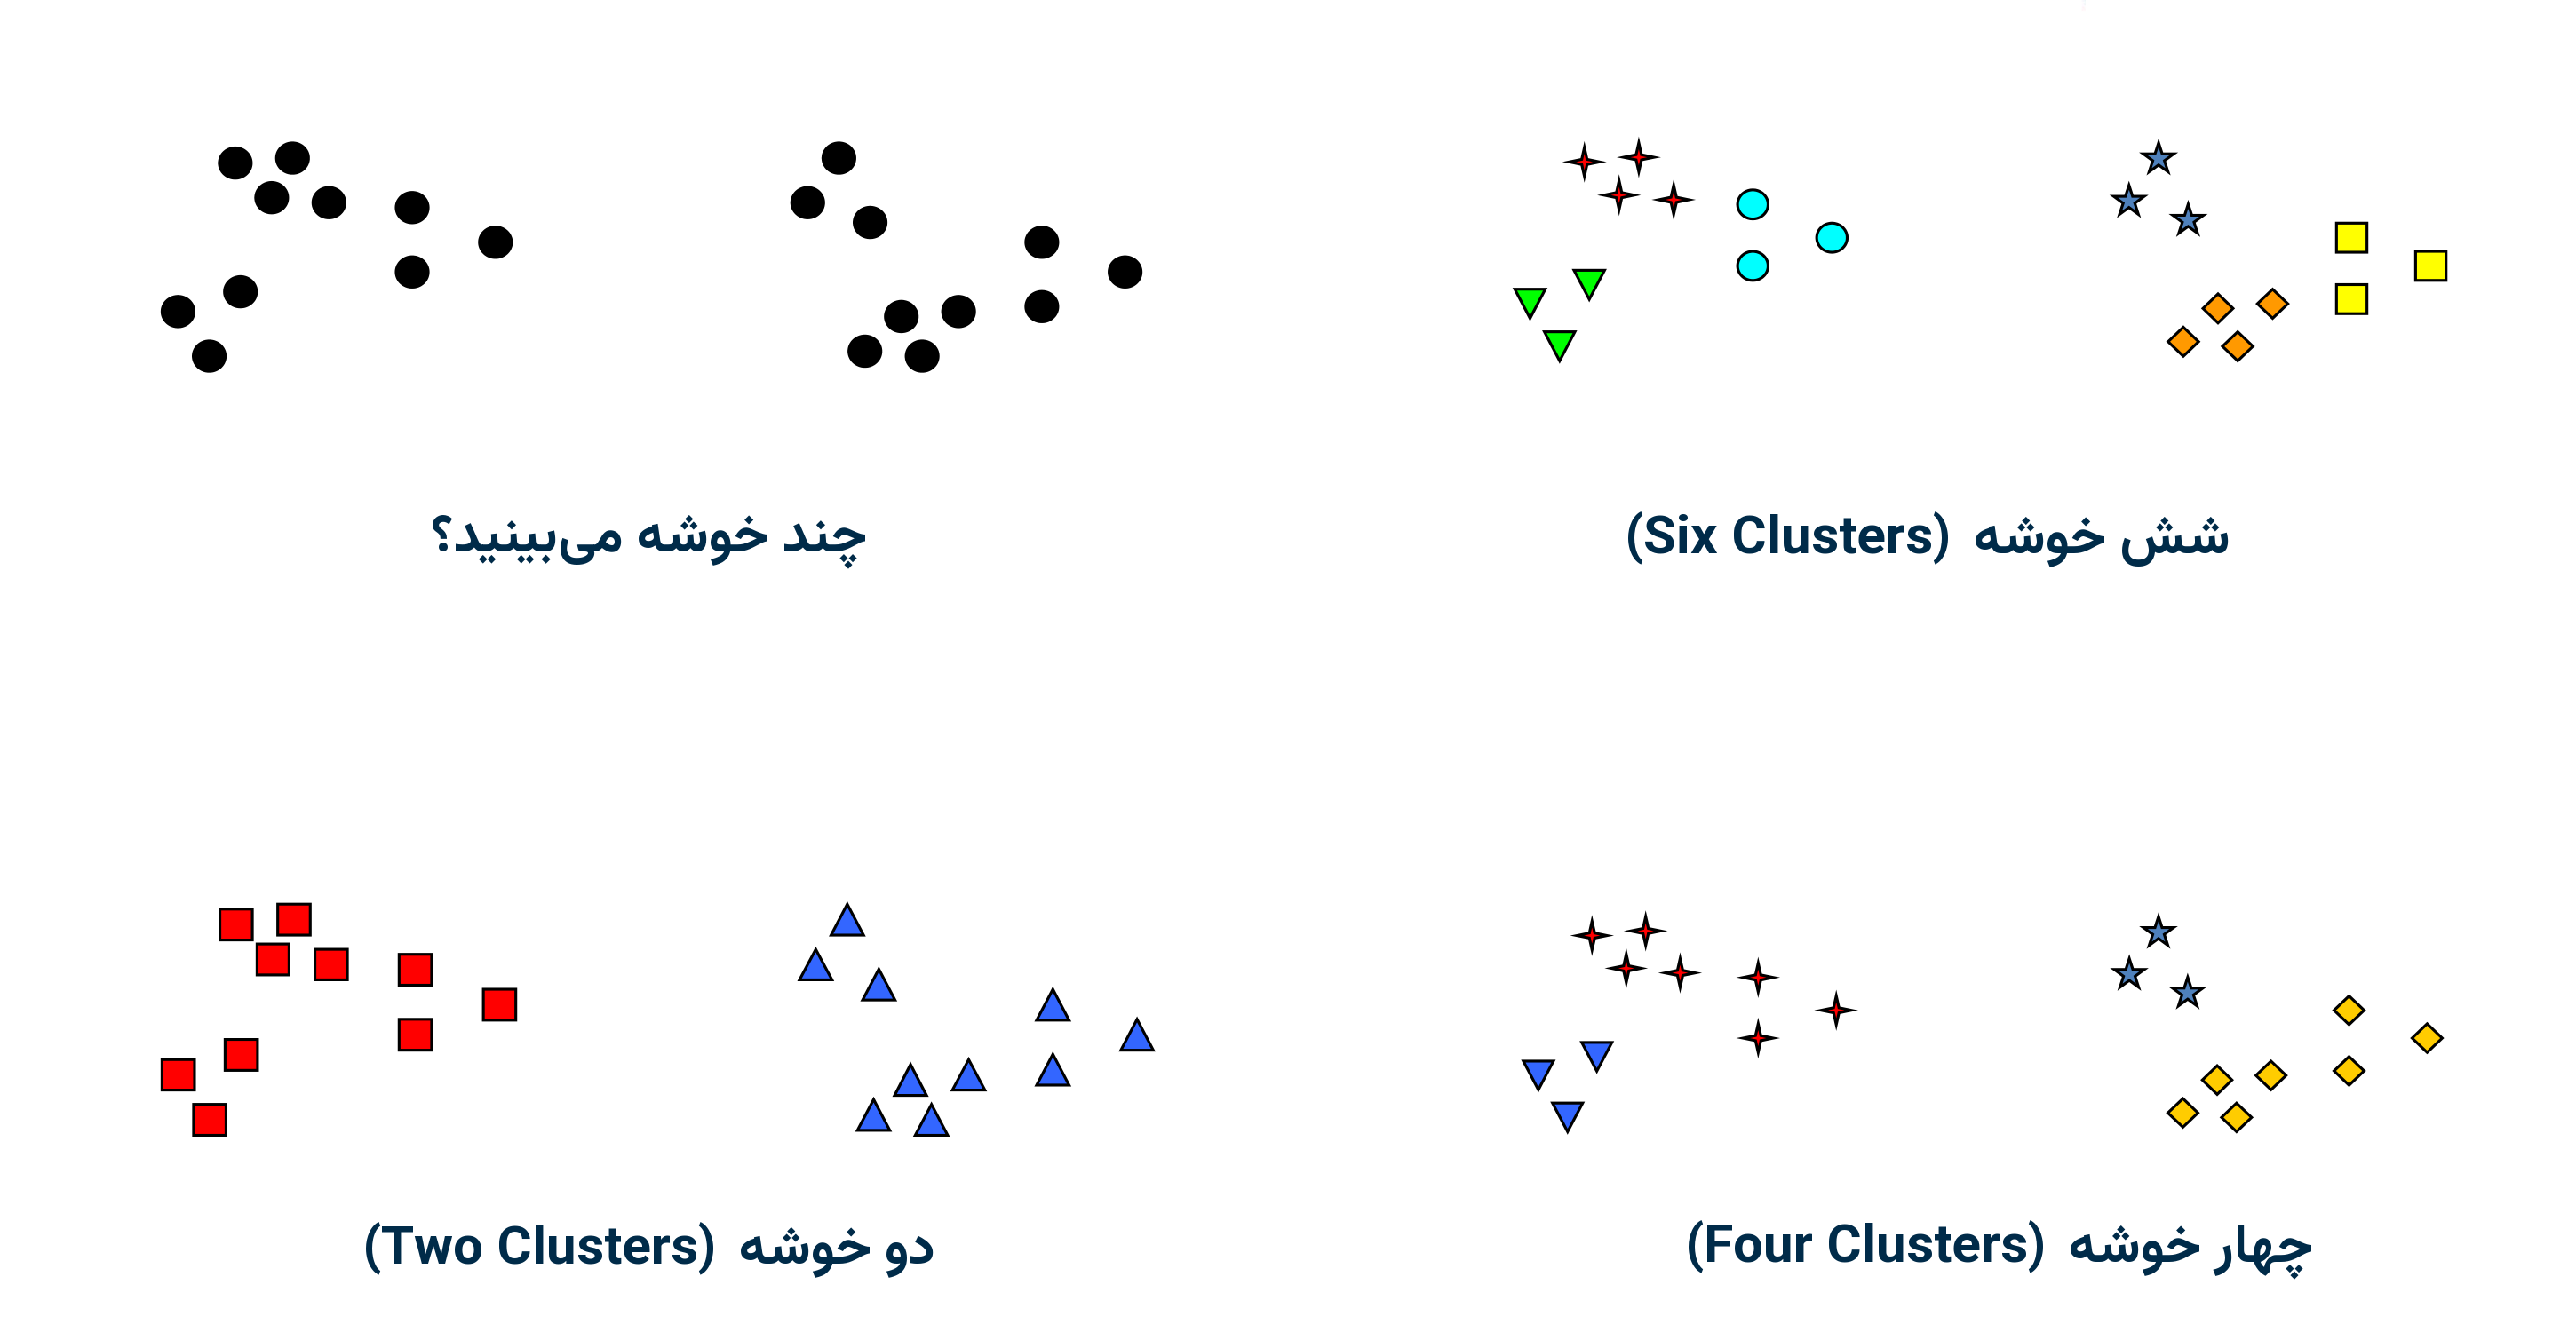
\includegraphics[width=0.85\textwidth,height=4.2cm,keepaspectratio]{images/slide07_points_persian.png}\\[0.15cm]
    {\fontsize{10.5}{13.5}\selectfont\color{mannheimblue}\textbf{مفید بودن یک خوشه‌بندی به هدف تحلیل بستگی دارد}}\\[0.05cm]
    {\fontsize{8.0}{10}\selectfont\color{gray}\lr{The usefulness of a clustering depends on the goal of the analysis}}
  \end{center}
\end{frame}

% Slide 8: Example Applications
\begin{frame}{نمونه‌هایی از کاربردهای خوشه‌بندی}{\lr{Example Applications}}
  \begin{columns}[T]
    \begin{column}{0.5\textwidth}
      \begin{itemize}
        \setlength{\itemsep}{6pt}
        \item \textbf{بخش‌بندی بازار:} \lr{(Market Segmentation)}
        \begin{itemize}
          \setlength{\itemsep}{2pt}
          \item هدف: شناسایی گروه‌هایی از مشتریان با رفتارهای مشابه.
          \item سطح تفکیک‌پذیری به نیاز کسب‌وکار بستگی دارد.
        \end{itemize}
        \item \textbf{تجارت الکترونیک:} \lr{(E-Commerce)}
        \begin{itemize}
          \setlength{\itemsep}{2pt}
          \item تطبیق و شناسایی پیشنهادات یک کالای یکسان در بازارهای برخط.
        \end{itemize}
        \item \textbf{تشخیص و پردازش تصویر:} \lr{(Image Recognition)}
        \begin{itemize}
          \setlength{\itemsep}{2pt}
          \item شناسایی بخش‌هایی از تصویر که به یک شیء واحد تعلق دارند.
        \end{itemize}
      \end{itemize}
    \end{column}
    \begin{column}{0.48\textwidth}
      \begin{center}
        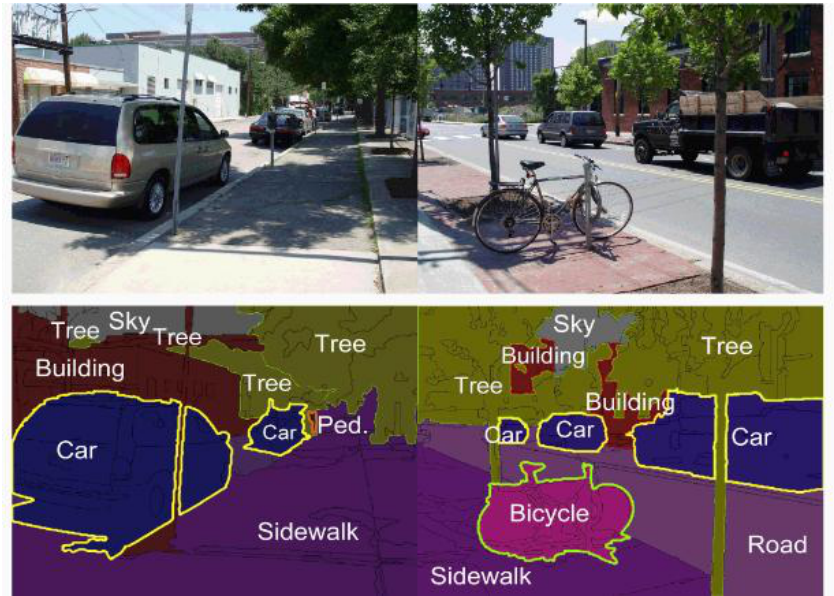
\includegraphics[width=0.45\textwidth,height=2.2cm,keepaspectratio]{images/slide08_marketing.png}\quad
        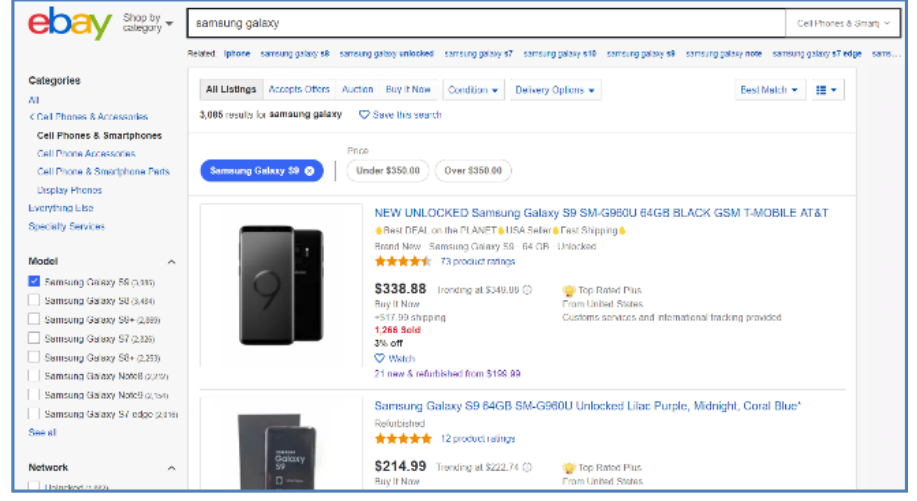
\includegraphics[width=0.45\textwidth,height=2.2cm,keepaspectratio]{images/slide08_genetics.png}\\[0.2cm]
        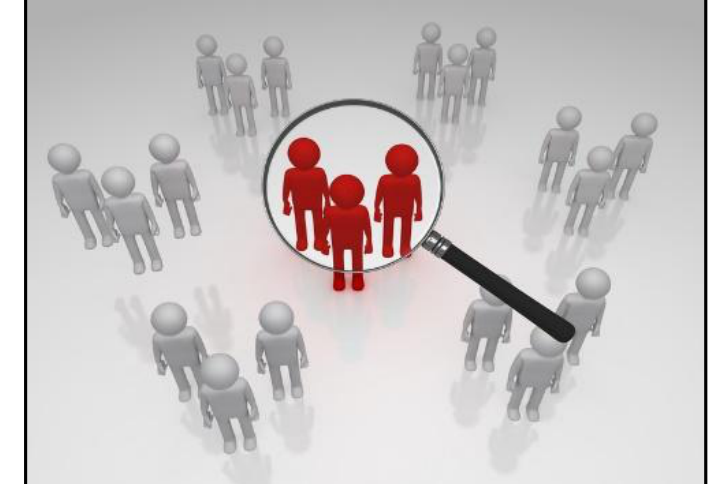
\includegraphics[width=0.7\textwidth,height=2.2cm,keepaspectratio]{images/slide08_astronomy.png}
      \end{center}
    \end{column}
  \end{columns}
\end{frame}
